\documentclass[tikz]{standalone}
%\documentclass{article}
%\usepackage{tikz}
\usepackage{wasysym}
\begin{document}
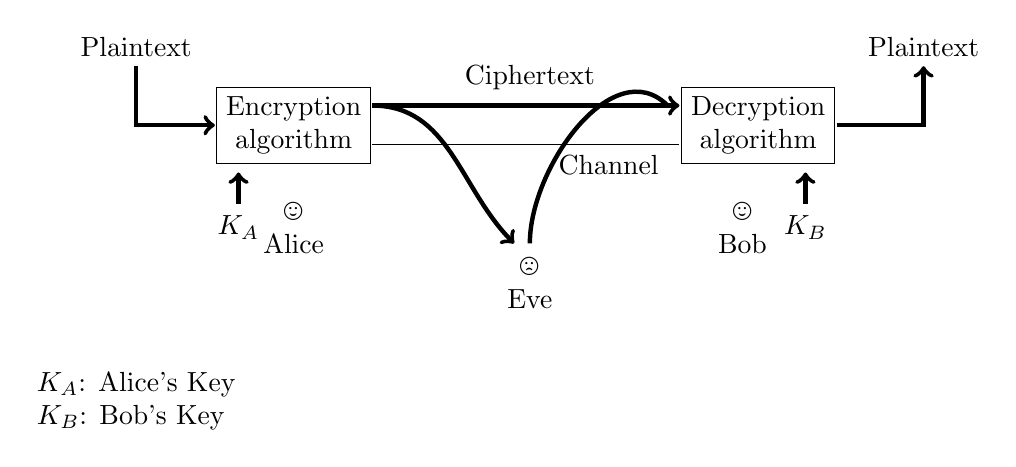
\begin{tikzpicture}
  %LEFT SIDE 
  \node[align=left] at (0, 4.5) {Plaintext};
  \draw [ultra thick, ->](0, 4.25) -- (0, 3.5) -- (1, 3.5);
  %%  \draw (1.1,5.5) rectangle(3.5,6.5);
  %%  \node [align=center] at (2.25, 6) {Encryption\\algorithm};
  \node [rectangle, draw, align=center] at (2,3.5) {Encryption\\algorithm};
  \draw [ultra thick, ->] (1.3, 2.5) -- (1.3, 2.9);
  \node [align=center] at (1.3, 2.2) {$K_A$};
  \node [align=center] at (2,2.2) {\smiley\\Alice};

  
  %CENTER  
  \draw [ultra thick, ->] (3, 3.75) -- (6.9, 3.75);
  \draw [thin] (3, 3.25) -- (6.9, 3.25);

  \node [align=center] at (5, 4.1) {Ciphertext};
  \node at (6, 3) {Channel};

  \draw [ultra thick, ->] (3, 3.75) to [out=0] (4.8, 2);
  \draw [ultra thick] (5, 2) to [out=90] (6.75,3.75);

  \node [align=center] at (5,1.5) {\frownie\\Eve};
  

  %RIGHT SIDE
  \draw [ultra thick, ->] (8.5,2.5) -- (8.5,2.9);
  \node [align=center] at (8.5, 2.2) {$K_B$};
  \node [align=center] at (7.7,2.2) {\smiley\\Bob};
    
  \node [rectangle, draw, align=center] at (7.9,3.5) {Decryption\\algorithm};

  \draw[ultra thick, ->] (8.9, 3.5) -- (10, 3.5) -- (10, 4.25);
  \node[align=left] at (10, 4.5) {Plaintext};
  
  %BOTTOM
  \node [align=left] at (0,0) {$K_A$: Alice's Key\\$K_B$: Bob's Key};

\end{tikzpicture}
\end{document}
